%% abtex2-modelo-artigo.tex, v-1.9.6 laurocesar
%% Copyright 2012-2016 by abnTeX2 group at http://www.abntex.net.br/ 
%%
%% This work may be distributed and/or modified under the
%% conditions of the LaTeX Project Public License, either version 1.3
%% of this license or (at your option) any later version.
%% The latest version of this license is in
%%   http://www.latex-project.org/lppl.txt
%% and version 1.3 or later is part of all distributions of LaTeX
%% version 2005/12/01 or later.
%%
%% This work has the LPPL maintenance status `maintained'.
%% 
%% The Current Maintainer of this work is the abnTeX2 team, led
%% by Lauro César Araujo. Further information are available on 
%% http://www.abntex.net.br/
%%
%% This work consists of the files abntex2-modelo-artigo.tex and
%% abntex2-modelo-references.bib
%%

% ------------------------------------------------------------------------
% ------------------------------------------------------------------------
%  abnTeX2: Modelo de Artigo Acadêmico em conformidade com
%  ABNT NBR 6022:2003: Informação e documentação - Artigo em publicação 
%  periódica científica impressa - Apresentação
% ------------------------------------------------------------------------
% ------------------------------------------------------------------------

\documentclass[
% -- opções da classe memoir --
article,			% indica que é um artigo acadêmico
11pt,				% tamanho da fonte
oneside,			% para impressão apenas no recto. Oposto a twoside
a4paper,			% tamanho do papel. 
% -- opções da classe abntex2 --
%chapter=TITLE,		% títulos de capítulos convertidos em letras maiúsculas
%section=TITLE,		% títulos de seções convertidos em letras maiúsculas
%subsection=TITLE,	% títulos de subseções convertidos em letras maiúsculas
%subsubsection=TITLE % títulos de subsubseções convertidos em letras maiúsculas
% -- opções do pacote babel --
english,			% idioma adicional para hifenização
brazil,				% o último idioma é o principal do documento
sumario=tradicional
]{abntex2}

\setlength\afterchapskip{\lineskip}

% ---
%  PACOTES
% ---

% ---
% Pacotes fundamentais 
% ---
\usepackage[dvipsnames]{xcolor}	% Controle das cores
\usepackage{lmodern}			% Usa a fonte Latin Modern
\usepackage[T1]{fontenc}		% Selecao de codigos de fonte.
\usepackage[utf8]{inputenc}		% Codificacao do documento (conversão automática dos acentos)
\usepackage{indentfirst}		% Indenta o primeiro parágrafo de cada seção.
\usepackage{nomencl} 			% Lista de simbolos
\usepackage{graphicx}			% Inclusão de gráficos
\usepackage{microtype} 			% para melhorias de justificação
\usepackage{glossaries}			% solução de glossário
\usepackage{nameref}			% referenciar também pelo nome
% ---

% ---
%  Pacotes de perfumaria
% ---
\usepackage{lipsum}				% para geração de dummy text
% ---

% ---
%  Pacotes de citações
% ---
\usepackage[brazilian,hyperpageref]{backref}	 % Paginas com as citações na bibl
\usepackage[alf]{abntex2cite}	% Citações padrão ABNT
% ---

% ---
%  Configurações do pacote backref
%  Usado sem a opção hyperpageref de backref
\renewcommand{\backrefpagesname}{Citado na(s) página(s):~}
% Texto padrão antes do número das páginas
\renewcommand{\backref}{}
% Define os textos da citação
\renewcommand*{\backrefalt}[4]{
	\ifcase #1 %
	Nenhuma citação no texto.%
	\or
	Citado na página #2.%
	\else
	Citado #1 vezes nas páginas #2.%
	\fi}%
% ---

% ---
%  Configurações do pacote glossaries
\renewcommand*{\glsclearpage}{}
% ---

% ---
%  Informações de dados para CAPA e FOLHA DE ROSTO
% ---
\titulo{Fichamentos para a disciplina de  Arranjos Institucionais e Marco Regulatório do Território}
\autor{Caio César Carvalho Ortega}
\local{São Bernardo do Campo, SP}
\data{26/11/2018}
% ---

% ---
%  Configurações de aparência do PDF final e informações do PDF
\makeatletter
\hypersetup{
	%pagebackref=true,
	pdftitle={\@title}, 
	pdfauthor={\@author},
	pdfsubject={Arranjos Institucionais},
	pdfcreator={LaTeX with abnTeX2},
	pdfkeywords={metropolização, metrópole, governança, metropolitana}, 
	colorlinks=true,		% false: boxed links; true: colored links
	linkcolor=Plum,			% color of internal links
	citecolor=Blue,			% color of links to bibliography
	filecolor=Red,			% color of file links
	urlcolor=Red,
	bookmarksdepth=4
}
\makeatother
% --- 

% ---
%  compila o glossário
% ---
%\makeglossaries

% \newglossaryentry{ex}{name={sample},description={an example}}

% ---

% ---
%  compila o indice
% ---
\makeindex
% ---

% ---
%  Altera as margens padrões
% ---
\setlrmarginsandblock{3cm}{3cm}{*}
\setulmarginsandblock{3cm}{3cm}{*}
\checkandfixthelayout
% ---

% --- 
%  Espaçamentos entre linhas e parágrafos 
% --- 

%  O tamanho do parágrafo é dado por:
\setlength{\parindent}{1.3cm}

%  Controle do espaçamento entre um parágrafo e outro:
\setlength{\parskip}{0.2cm}  % tente também \onelineskip

%  Espaçamento simples
\SingleSpacing

% ----
%  Início do documento
% ----
\begin{document}
	
	% Seleciona o idioma do documento (conforme pacotes do babel)
	%\selectlanguage{english}
	\selectlanguage{brazil}
	
	% Retira espaço extra obsoleto entre as frases.
	\frenchspacing 
	
	% ----------------------------------------------------------
	%  ELEMENTOS PRÉ-TEXTUAIS
	% ----------------------------------------------------------
	
	%---
	%
	% Se desejar escrever o artigo em duas colunas, descomente a linha abaixo
	% e a linha com o texto ``FIM DE ARTIGO EM DUAS COLUNAS''.
	% \twocolumn[    		% INICIO DE ARTIGO EM DUAS COLUNAS
	%
	%---
	% página de titulo
	\maketitle
	
	% ---
	% Título e resumo em língua estrangeira
	% ---

	% ----------------------------------------------------------
	%  ELEMENTOS TEXTUAIS
	% ----------------------------------------------------------
	\textual
	
	% ----------------------------------------------------------
	% Introdução
	% ----------------------------------------------------------
	
	\section*{Prólogo}
	\addcontentsline{toc}{section}{Prólogo}
	
	O propósito do presente trabalho é realizar dois breves fichamentos para a disciplina de Arranjos Institucionais e Marco Regulatório do Território (BH1343), constituídas de um parágrafo cada.
	
	\section{Fichamentos}
	
	\subsection{Primeiro fichamento}
	
	O autor pretende discutir a relação entre o território e o arranjo federativo com vistas ao cumprimento dos objetivos fundamentais da CF/88\footnote{Constituição Federal da República Federativa do Brasil}, como o combate e erradicação da pobreza e o desenvolvimento nacional, sendo para tanto a estrutura político administrativa dividida em três poderes como parte de uma união indissolúvel: (i) União; (ii) estados e o DF\footnote{Distrito Federal} e; (iii) municípios \cite[p. 89]{mendes2012}, sendo feito um recorte voltado à problemática do desenvolvimento da região Nordeste.
	
	Para o autor o território é um mecanismo capaz de dar coesão às políticas públicas que deverão partir das esferas, de forma a orientar os instrumentos, diferindo do panorama construído nos últimos 50 anos, no qual houve desarticulação entre objetivos e instrumentos \cite[p. 90]{mendes2012}. Especificamente sobre os instrumentos, \citeonline[p. 90]{mendes2012} debruça-se sobre os de ação pública. \citeonline{mendes2012} salienta ainda que não há consenso quanto ao federalismo brasileiro e o modelo descentralizador da CF/88. Enumera os seguintes aspectos:
	
	\begin{citacao}
		``(\dots) a redução da capacidade financeira e administrativa da União e mesmo dos estados de prover serviços públicos adequados; a falta de 	planejamento no processo de redefinição das atribuições entre as diversas esferas 		de governo; o interesse político consciente de delegar aos estados e municípios 	mais responsabilidades, dada, em particular no último caso, a sua proximidade 	com a comunidade; a necessidade de aumentar as responsabilidades estaduais e municipais na provisão de serviços públicos, tendo em vista o ganho dos estados e municípios com a descentralização fiscal; a identificação dos problemas associados à escala de determinados tipos de serviços públicos (\dots)'' \cite[p. 90]{mendes2012}
	\end{citacao}
	
	Utilizando fontes secundárias, \citeonline[p. 93]{mendes2012} aponta que ``em determinadas situações ou em função de certas condições e	características socioeconômicas, a descentralização federativa, em termos de definição de competências públicas, é relevante para o atendimento da demanda local da sociedade'', realizando para tanto uma reflexão a partir do período \textit{café com leite}, quando a capital estava no Rio de Janeiro e os estados de Minas Gerais e São Paulo conseguiam beneficiar sua estrutura produtiva em detrimento do restante do país, além de fontes secundárias. No entanto, \citeonline[p. 93]{mendes2012} não deixa de apontar a existência de uma controvérsia teórica ligada à visão do gasto público, que posteriormente levou a estratégicas de planejamento no âmbito do estado, notadamente centralizadoras no caso do Brasil dos anos 1950 \cite[p. 94]{mendes2012}.
	
	O seguinte trecho da obra resume de maneira formidável o desafio do desenvolvimento brasileiro e da própria configuração institucional, sendo que as duas coisas estão imbricadas:
	
	\begin{citacao}
		``Se o contexto teórico moderno sobre o papel do Estado e do mercado no desenvolvimento nacional está em aberto, a experiência empírica moderna demonstra a incapacidade de grande parcela dos municípios brasileiros em, de um lado, ter capacidade arrecadatória própria, ficando, assim, dependentes de transferências estaduais e federais e, de outro, prover bens e serviços públicos adequados para sua população local ou de criarem, “a partir de baixo”, uma visão de um país integrado regional e nacionalmente. Estes mesmos municípios são fortemente dependentes de recursos 	tributários federais e estaduais, por não contarem com uma base contributiva autônoma, seja em virtude da pequena população, seja por causa de estruturas produtivas deficientes. Ao mesmo tempo, de um modo inverso, mas complementar, existe a constatação empírica de que o governo federal, sozinho ou de forma exclusiva, não tem condições de articular, conciliar e orientar todos os interesses envolvidos na escolha de uma ação pública que atente para as especificidades de demandas das sociedades (heterogêneas) regionais, estaduais e locais.'' \cite[p. 94]{mendes2012}
	\end{citacao}
	
	Não obstante, o \citeonline[p. 95]{mendes2012} considera que as figuras regionais em conjunto com outros instrumentos normativos, tais como consórcios, APLs\footnote{Arranjos Produtivos Locais} e RIDEs\footnote{Regiões Integradas de Desenvolvimento}, a luz da CF/88, contribuem ``para que exista a possibilidade de conciliar, dentro de uma visão e de um planejamento territorial, os principais instrumentos das diversas esferas federativas para o objetivo comum de desenvolvimento regional e nacional''.
	
	\begin{figure}[htb]
		\centering
		\caption{Elementos de planejamento: diagnóstico, meios e objetivos}
		\label{fig:mendes2010_pag0098}
		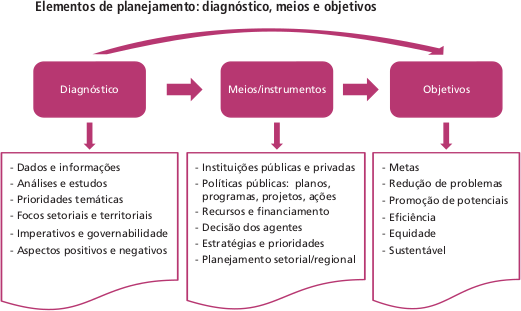
\includegraphics[width=0.7\linewidth]{img/mendes2010_pag0098}
		\legend{Extraído de: \citeonline[p. 96]{mendes2012}. Fonte: \citeonline{buarque2003}}
	\end{figure}

	Na \autoref{fig:mendes2010_pag0098} (\nameref{fig:mendes2010_pag0098}), \citeonline{mendes2012} sumariza o método proposto e adotado no capítulo lido. Em seguida, aprofunda o diagnóstico, principalmente de caráter econômico e finaliza apontando o papel preponderante das cidades no processo, afirmando que ``não há planejamento razoável que dê conta de articular e integrar ações de 5.565 municípios, nas 27 Unidades Federativas, na sua maioria pequenos núcleos urbanos com baixa autonomia para gerar dinâmica econômica e dotar a sociedade local com autonomia própria'' \cite[p. 101]{mendes2012}.
	
	Em seguida, o \citeonline[p. 101]{mendes2012} passa a se voltar para os instrumentos. É oportuna a menção ao IBGE\footnote{Instituto Brasileiro de Geografia e Estatística}, ligada ao estudo ``Regiões de Influência das Cidades – REGIC'', o qual trabalha com uma noção de centralidades e a influência exercida por estas. Trata-se de um ponto nevrálgico para que \citeonline{mendes2012} construa o arcabouço teórico necessário para sustentar sua visão sobre a região Nordeste. Para \citeonline[p. 104]{mendes2012}, ``essa distribuição de papéis urbano-regionais, que podem ser explicitados por meio de “consórcios ou arranjos federativos” dentro de cada região (grupamentos de municípios), deve ser combinada e apoiada, ainda,
	na estrutura institucional e técnico-científica e produtiva interna''. Dada a baixa institucionalidade local dos APLs \cite[p. 106]{mendes2012}, o autor sugere articular a noção de redes urbanas regionais, cidades-núcleo, estrutura produtiva (sem se limitar apenas a setores produtivos) e instituições públicas e seus instrumentos, processo que sintetiza no parágrafo abaixo:
	
	\begin{citacao}
		``A visão territorial do papel de cidades-núcleo e da rede urbana regional pode ser complementada por uma concepção que integre, no território, a estrutura produtiva (não somente os setores produtivos) e as instituições (e seus instrumentos) públicas e/ou privadas capazes de não somente estudar ou pesquisar os	problemas da região, mas também intervir de maneira articulada e coordenada. (\dots)'' \cite[p. 106]{mendes2012}
	\end{citacao}
	
	Sugere ainda conciliar consumo massificado com produção, educação e geração de empregos massificados, com vistas à manutenção de uma ``dinâmica equilibrada da matriz produtiva regional''. \cite[p. 107]{mendes2012}.
	
	A conclusão de \citeonline[p. 107]{mendes2012} aponta que há uma assimetria entre os avanços do Nordeste, dada sua participação no PIB\footnote{Produto Interno Bruto} nacional estabilizada em aproximadamente 13\%, acabam por serem mitigados por uma situação estrutural permanente. Entre os fatores que contribuem para um cenário tão crítico, estão ``gastos públicos \textit{per capita} inferiores ao nível nacional em setores fundamentais, como educação e saúde'' \cite[p. 107]{mendes2012}. \citeonline[p. 108]{mendes2012} defende a utilização do planejamento como elemento estruturador de uma agenda que gere emprego e renda salarial a partir de um modelo de produção em massa (ou seja, incentivos e financiamentos à produção regional). Sugere ainda diagnósticos que estejam calcados na `` identificação dos elementos ou instrumentos causais capazes de modificar a realidade regional'', em oposição a meras correlações implícitas \cite[p. 108]{mendes2012}. Finalmente, \citeonline[p. 108--109]{mendes2012} assinala para a necessidade de rediscutir a tomada de decisões e consolidar um anova agenda regional de desenvolvimento, modificando a lógica orçamentária do federalismo em vigência, bem como de associar o orçamento rediscutido a um planejamento estratégico e impactos dos mecanismos e instrumentos, com metas e objetivos em múltiplas escalas.
	
	\subsection{Segundo fichamento}
	
	\subsubsection{Municípios e regiões metropolitanas na federação brasileira}
	
	\citeonline[p. 51--52]{machado2009} começa destacando o pioneirismo brasileiro em dotar o município de autonomia, enumerando três elementos que consolidam um panorama \textit{de facto} único no Brasil:
	
	\begin{enumerate}
		\item Edição das próprias leis via Câmara Municipal (poder legislativo);
		\item Elaboração e aprovação autônoma da Lei Orgânica, sem necessidade de consultar entes federativos superiores (auto-organização local, portanto);
		\item Autonomia financeira local, por meio do estabelecimento e arrecadação autônoma de tributos.
	\end{enumerate}
	
	Tais fatores se somam à padronização institucional da figura regional municipal, ``sem distinções de espécies e escalas de governos locais'' \cite[p. 52]{machado2009}, embora exista um contraste no que diz respeito à discrepância de porte dos municípios \cite[p. 53]{machado2009}. Surpreende a comparação com a França, que possui 36 mil governos locais organizados ante os 6 mil municípios do Brasil \cite[p. 53]{machado2009}.
	
	Realizando uma contextualização histórica, \citeonline{machado2009} aponta que a padronização dos municípios é uma herança colonial, recrudescida com a CF/88, cujo ``grande realce'' nada mais é do que o ``cume de um processo histórico de origem secular'' \cite[p. 55]{machado2009}, no entanto, a autonomia sofreu revezes durante o Estado Novo varguista, cuja luta dos chamados municipalistas se fez e se faz sentir até os dias de hoje na Constituição \cite[p. 55]{machado2009}. O autor ainda contextualiza o funcionamento dos entes, explicando que apenas prefeito e vereadores são escolhidos por sufrágio universal, bem como que a União e municípios concentram competências expressamente definidas na Constituição, enquanto os estados-membros ficam com as competências residuais \cite[p. 56-57]{machado2009}.
	
	O autor discute então o impasse ligado à gestão metropolitana no Brasil, apontando que uma cidade não pode, salvo casos excepcionais, investir em outra, o que torna a situação particularmente difícil para cidades que não possuem receitas suficientes advindas da tributação de patrimônio e atividades produtivas, ficando dependentes da União e estados \cite[p. 57]{machado2009}. Os municípios acumulam fracassos na realização de acordos formais e informais entre si, prevalecendo a competitividade em oposição à cooperação \cite[p. 57]{machado2009}. Os casos mais positivos são, em geral, fruto de esforços da União e dos estados, que estabelecem marcos regulatórios que orientam os municípios (exemplo: consórcios) \cite[p. 58]{machado2009}, porém, \citeonline[p. 58]{machado2009} salienta que não há obrigatoriedade para exigir certos tipos de posturas cooperativas, incluindo a formação e participação em consórcios e associações, diferindo do que acontece em Portugal e Alemanha.
	
	Ainda sobre a gestão metropolitana, \citeonline[p. 58]{machado2009} aponta que a luz da CF/88, há a possibilidade de que estados criem aglomerações urbanas e microrregiões, além das já existentes regiões metropolitanas, também reconhecidas pelo texto da Carta. \citeonline[p. 59]{machado2009} aponta ainda que não há total consenso na sociedade civil organizada quanto às funções públicas de interesse comum que envolvem a atuação dos estados-membros em assuntos ligados a múltiplos municípios. Trata-se, no entanto, de uma preocupação que é, segundo o autor, aplacada pelo surgimento do Ministério das Cidades, ainda que existam controvérsias no caso de regiões metropolitanas, como acontece com o saneamento \cite[p. 60--61]{machado2009}.
	
	Há, segundo \citeonline[p. 62]{machado2009}, um \textbf{custo transacional} para os estados, visto que a participação dos municípios em regiões metropolitanas é compulsória, produzindo um hiato entre os papéis da União e dos municípios. Há exemplos de gestão verticalizada, porém, como o caso dos Comitês de Bacia Hidrográficas \cite[p. 62]{machado2009}, que o autor considera a alternativa mais defendida no meio político e acadêmico \cite[p. 63]{machado2009}. Juridicamente, os instrumentos existentes para a cooperação intergovernamental de vínculo facultativo são os convênios e consórcios \cite[p. 63]{machado2009}; os primeiros são de curta duração, mais precários e com pouco impacto na autonomia dos envolvidos, o que por outro lado dificulta ir além do imediatismo e compor um planejamento metropolitano de maior abrangência e duração \cite[p. 64]{machado2009}; os segundos, ainda que sejam menos robustos do que estruturas de organização e planejamento mais duradouras, ainda assim são menos dispendiosos, baseados em acordos bem específicos e com permissividade para que os envolvidos sigam negociando sua lealdade ``no varejo'' \cite[p. 63]{machado2009}, por outro lado, possuem pessoa jurídica e estão dotados de corpo funcional e patrimonial próprios, o que contribui para dar um verniz mais consistente às bases de cooperação intergovernamental \cite[p. 64]{machado2009}.
	
	Como explica \citeonline[p. 65--66]{machado2009}, os consórcios adquirem um marco regulatório mais robusto quando os então membros do Consórcio do Grande ABC entregam a \textit{Carta do ABC} ao então presidente da república, Luís Inácio Lula da Silva, fortalecendo a emenda 19/1998, que definiu a redação do Art. 241 da CF/88, a partir do PL\footnote{Projeto de Lei} 3.884/2004, que acabou precisando de um substitutivo redigido pela ``Bancada da Saúde'', mais experiente com o tipo de arranjo em questão, sendo este aprovado pelo Congresso e sancionado por Lula \cite[p. 67]{machado2009}.
	
	\subsubsection{A trajetória do Grande ABC paulista}
	
	Com a proposta de fazer uma comparação entre a RMBH\footnote{Região Metropolitana de Belo Horizonte} e RMSP\footnote{Região Metropolitana de São Paulo}, \citeonline[p. 100]{machado2009} inicia com uma contextualização sobre a trajetória, que remonta ao Consórcio Intermunicipal das Bacias do Alto Tamanduateí e Billings, em 1990. Quando o autor escrevia, o consórcio era formado por sete municípios da RMSP: Santo André, São Bernardo, São Caetano, Diadema, Mauá, Ribeirão Pires e Rio Grande da Serra. A articulação regional envolve três estruturas institucionais: (i) Consórcio Intermunicipal; (ii) Câmara Regional e; (iii) Agência de Desenvolvimento Econômico do Grande ABC.
	
	A contextualização feita por \citeonline[p. 100]{machado2009} avança a medida que passa a observar o sistema de gestão vertical-compulsório da própria RMSP, institucionalizada em 1973. \citeonline[p. 101]{machado2009} aponta que o sistema de gestão foi enfraquecido com a redemocratização, tanto que os antigos órgãos colegiados da década de 1970 nunca mais foram convocados após a redemocratização. O que o GESP\footnote{Governo do Estado de São Paulo} tem mantido são órgãos próprios de vocação metropolitana, como Emplasa\footnote{Empresa de Planejamento Metropolitano de São Paulo S.A.}, EMTU\footnote{Empresa Metropolitana de Transportes Urbanos de São Paulo}, CPTM\footnote{Companhia Paulista de Trens Metropolitanos} e Sabesp\footnote{Companhia de Saneamento Básico de São Paulo S.A.}.
	
	A RMSP resistiu mais ao municipalismo do que a RMBH, pois a LC 760/94 manteve um conselho de desenvolvimento com composição paritária entre estado e municípios, enquanto a RMBH adota uma Assembleia Metropolitana que é, em suma, municipalista \cite[p. 101]{machado2009}. O cenário não significa que não ocorram conflitos e problemas, dentro os quais, podem ser elencados com base em \citeonline[p. 102]{machado2009}:
	
	\begin{itemize}
		\item Disputas pelo controle dos recursos hídricos, com batalhas judiciais envolvendo municípios e a Sabesp;
		\item O não-envolvimento da Emplasa na implementação de políticas públicas, ainda que esta siga planejando a RMSP e desde 1994 conte com um plano para detecção de carências e potencialidades;
		\item Não implementação da estrutura precista em lei;
		\item Ausência de uma política regional;
		\item Recursos financeiros rarefeitos;
		\item Disputas político-partidárias;
		\item Conflitos de juridição entre as três esferas;
		\item Desigualdade econômica entre regiões.
	\end{itemize}
	
	No caso do governo estadual, os entraves acabam levando à setorialização e à redução da escala \cite[p. 102]{machado2009}. Em seguida \citeonline[p. 103--115]{machado2009} se volta a fazer uma espécie de balanço da experiência do Grande ABC:
	
	\begin{itemize}
		\item Registrado como sociedade civil de direito privado, com os sete municípios da região como sócios;
		\item Presidência concebida para ser rotativa: mandatos de um ano, exercidos pelos prefeitos dos municípios-membros;
		\item Recursos financeiros definidos a partir de cotas de contribuição anual proporcionais às receitas dos municípios;
		\item Natureza jurídica de direito privado impede a execução direta de programas e projetos de interesse comum, exceto pela contratação de estudos;
		\item Natureza jurídica de direito comum impede que o Governo Federal seja avalista e viabilize a contratação de financiamentos externos, pois a personalidade jurídica não dá garantias de crédito (caixa próprio);
		\item Firmou-se como entidade de articulação de políticas públicas integradas, com grupos temáticos compostos por técnicos das prefeituras dos municípios-membros;
		\item Assiduidade das reuniões sujeita ao projeto político dos prefeitos eleitos, com histórico de esvaziamento por políticos de perfil conservador;
		\item O consórcio foi pivô de um esforço regional com o Fórum da Cidadania durante a crise econômica enfrentada pelos municípios em 1994, promovendo a conscientização da população em prol da eleição de políticos locais para os cargos de deputado federal e estadual;
		\item Em 1997 surge a Câmara do Grande ABC, um fórum intergovernamental e social de planejamento;
		\item Estreita relação entre o Consórcio e grupos da sociedade civil organizada ligados aos trabalhadores, notadamente de certos setores produtivos;
		\item Processo de execução dos acordos da Câmara do Grande ABC tem feição caleidoscópica, ou seja, diversos atores (públicos ou privados) podem ser responsáveis pela implementação;
		\item Agência de Desenvolvimento do Grande ABC foi fruto de um acordo, bem como também foram o plano de macrodrenagem, o planejamento do sistema viário em parceria com a Emplasa e o plano dos transportes de massa em convênio com a EMTU, além de uma parceria com a CPTM para modernização do sistema de transportes;
		\item Falta de orçamento e estrutura própria torna as ações reféns de dotações específicas e de diferentes fontes, que nem sempre são executadas;
		\item Discussão em relação à guerra fiscal, afetada pela autonomia e assimetria do poder político entre os municípios-membros;
		\item Demonstrações dos prefeitos dão indícios de que o interesse local prevalece sobre o regional em casos de confronto;
		\item Atomização nos serviços de caráter metropolitano, como saneamento e transportes, com os municípios mantendo estruturas próprias;
		\item Estrutura do Consórcio voltada para as despesas administrativas e do fórum de debates, com apenas 12 funcionários, reitera perfil de interlocução e não de execução;
		\item O limite de atuação do Consórcio é a própria autonomia municipal, o que acaba criando forte dependência com relação aos governos federal e estadual;
		\item Custos de transação podem ser reduzidos por relações de confiança, como a ocorrida entre o então prefeito de Santo André, Celso Daniel e o então governador do Estado de São Paulo, Mário Covas;
		\item Institucionalidade limitada exige boas relações interpessoais entre políticos para que a cooperação logre êxito;
		\item Consórcio com perfil de lobista e não de gestor.
	\end{itemize}
	
	Finalmente, \citeonline[p. 115]{machado2009} aposta em custos elevados para o rompimento de municípios em consórcios como o do Grande ABC, além de sugerir que ``a exigência de equipe técnica aprovada em concurso, o fluxo constante de recursos e as restrições para a desativação irresponsável da associação poderão significar maior autonomia para o consórcio e menor para os municípios'' \cite[p. 116]{machado2009}. Ademais, o perfil de liderança do finado Celso Daniel não teve equivalentes, sendo substituído por disputas pelo controle da entidade \cite[p. 116]{machado2009}, o que, entretanto, sinaliza uma certa importância e peso político  da entidade, para o autor, há a necessidade de ``admitir a pluralidade e o conflito não como anomalias, mas sim como inerentes aos jogos federativos''.
	
	% ---
	% Finaliza a parte no bookmark do PDF, para que se inicie o bookmark na raiz
	% ---
	\bookmarksetup{startatroot}% 
	% ---
	
	% ----------------------------------------------------------
	%  ELEMENTOS PÓS-TEXTUAIS
	% ----------------------------------------------------------
	\postextual
	
	% ----------------------------------------------------------
	% Referências bibliográficas
	% ----------------------------------------------------------
	\bibliography{fontes}
	
	% ----------------------------------------------------------
	% Glossário
	% ----------------------------------------------------------
	% Consultar manual da classe abntex2 para orientações sobre o
	% uso do glossário.
	\renewcommand{\glossaryname}{Glossário}
	%\renewcommand{\glossarypreamble}{Esta é a descrição do glossário.\\ \\}
	\renewcommand*{\glsseeformat}[3][\seename]{\textit{#1}
		\glsseelist{#2}}
	
	% ---
	% Traduções para o ambiente glossaries
	% ---
	\providetranslation{Glossary}{Glossário}
	\providetranslation{Acronyms}{Siglas}
	\providetranslation{Notation (glossaries)}{Notação}
	\providetranslation{Description (glossaries)}{Descrição}
	\providetranslation{Symbol (glossaries)}{Símbolo}
	\providetranslation{Page List (glossaries)}{Lista de Páginas}
	\providetranslation{Symbols (glossaries)}{Símbolos}
	\providetranslation{Numbers (glossaries)}{Números} 
	% ---
	
	% ---
	% Imprime o glossário
	% ---
	%\cleardoublepage
	%\phantomsection
	%\addcontentsline{toc}{section}{\glossaryname}
	%\glossarystyle{index}
	% \glossarystyle{altlisthypergroup}
	% \glossarystyle{tree}
	%\printglossaries
	
	% ----------------------------------------------------------
	% Apêndices
	% ----------------------------------------------------------
	
	% ---
	% Inicia os apêndices
	% ---
	%	\begin{apendicesenv}
	%		
	%		% ----------------------------------------------------------
	%		\chapter{Nullam elementum urna vel imperdiet sodales elit ipsum pharetra ligula
	%			ac pretium ante justo a nulla curabitur tristique arcu eu metus}
	%		% ----------------------------------------------------------
	%		\lipsum[55-57]
	%		
	%	\end{apendicesenv}
	% ---
	
	% ----------------------------------------------------------
	% Anexos
	% ----------------------------------------------------------
	%	\cftinserthook{toc}{AAA}
	% ---
	% Inicia os anexos
	% ---
	%\anexos
	%	\begin{anexosenv}
	%		
	%		% ---
	%		\chapter{Cras non urna sed feugiat cum sociis natoque penatibus et magnis dis
	%			parturient montes nascetur ridiculus mus}
	%		% ---
	%		
	%		\lipsum[31]
	%		
	%	\end{anexosenv}
	
\end{document}
